El problema más típico que lleva a la búsqueda binaria es el siguiente. Te dan una matriz ordenada $A_0 \leq A_1 \leq \dots \leq A_{n-1}$, comprobar si $k$ está presente dentro de la secuencia. La solución más sencilla sería comprobar cada elemento uno por uno y compararlo con $k$ (la llamada búsqueda lineal). Este enfoque funciona en $O(n)$, pero no utiliza el hecho de que la matriz esté ordenada.

% TODO: \usepackage{graphicx} required
\begin{figure}[h!]
	\centering
	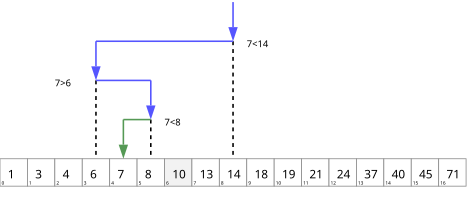
\includegraphics[width=0.7\linewidth]{img/Binary_Search_Depiction}
	\label{fig:binarysearchdepiction}
\end{figure}

Ahora supongamos que conocemos dos índices $L <R$ tal que $A_L \leq k \leq A_R$. Como la matriz está ordenada, podemos deducir que $k$ cualquiera de los dos ocurre entre $A_L, A_{L+1}, \dots, A_R$ o no aparece en la matriz en absoluto. Si elegimos un índice arbitrario $M$ tal que $L <M <R$ y comprobar si $k$ es menor o mayor que $A_M$. Tenemos dos casos posibles:

\begin{itemize}
	\item $A_L \leq k \leq A_M$. En este caso, reducimos el problema de $[L, R]$ a $[L,M]$.
	\item $A_M \leq k \leq A_R$. En este caso, reducimos el problema de $[L, R]$ a $[M,R]$.
\end{itemize}

Cuando es imposible elegir $M$, Eso es cuando $R = L + 1$, comparamos directamente $k$ con $A_L$ y $A_R$. De lo contrario, querríamos elegir $M$ de tal manera que reduzca el segmento activo a un solo elemento lo más rápidamente posible en el peor de los casos.

Dado que en el peor de los casos siempre reduciremos a un segmento mayor de $[L,M]$ y $[M,R]$. Así, en el peor de los casos la reducción sería de $R-L$ a $\max(M-L, R-M)$. Para minimizar este valor, debemos elegir $M \approx \frac{L+R}{2}$, entonces:

$$M-L \approx \frac{R-L}{2} \approx R-M.$$

En otras palabras, desde la perspectiva del peor de los casos, lo óptimo es elegir siempre $M$ en el medio de $[L, R]$ y dividirlo por la mitad. Por lo tanto, el segmento activo se reduce a la mitad en cada paso hasta que alcanza el tamaño $1$. Entonces, si el proceso necesita $h$ pasos, al final reduce la diferencia entre $R$ y $l$ de $R-L$ a $\frac{R-L}{2^h} \approx 1$, dándonos la ecuación $2^h \approx R-L$.

Tomando $\log_2$ en ambos lados, obtenemos $h \approx \log_2(R-L) \in O(\log n)$.

El número logarítmico de pasos es drásticamente mejor que el de la búsqueda lineal. Por ejemplo, para $n \approx 2^{20} \approx 10^6$ necesitarías realizar aproximadamente un millón de operaciones para la búsqueda lineal, pero solo alrededor $20$ operaciones con la búsqueda binaria.

\subsubsection{Límite inferior y límite superior}

A menudo es conveniente encontrar la posición del primer elemento que no sea menor que $k$ (llamado límite inferior de $k$ en la matriz) o la posición del primer elemento que es mayor que $k$ (llamado límite superior de $k$) en lugar de la posición exacta del elemento.

Juntos, los límites inferior y superior producen un medio intervalo posiblemente vacío de los elementos de la matriz que son iguales a $k$. Para comprobar si $k$ está presente en la matriz, es suficiente encontrar su límite inferior y verificar si el elemento correspondiente equivale a $k$.

La explicación anterior proporciona una descripción aproximada del algoritmo. Para los detalles de implementación, necesitaríamos ser más precisos.

Mantendremos un par $L <R$ tal que $A_L \leq k < A_R$. Lo que significa que el intervalo de búsqueda activa es $[L, R)$. Usamos medio intervalo aquí en lugar de un segmento. $[L, R]$ ya que resulta que requiere menos trabajo de caso.

Cuando $R = L+1$, podemos deducir de las definiciones anteriores que $R$ es el límite superior de $k$. Es conveniente inicializar $R$ con índice pasado el final, es decir $R=n$ y $l$ con índice antes del comienzo, es decir $L=-1$. Está bien siempre y cuando nunca evaluemos $A_L$ y $A_R$ en nuestro algoritmo directamente, tratándolo formalmente como $A_L = -\infty$ y $A_R = +\infty$.

Finalmente, para ser específico sobre el valor de $M$ elegimos, nos quedaremos con $M = \lfloor \frac{L+R}{2} \rfloor$.